\section{Intro}
\begin{frame}{Motivation}
	\begin{columns}[T]
		\begin{column}{0.45\textwidth}
			Festplatten-Geschwindigkeit:
			
\includegraphics[width=0.75\textwidth]{pics/slow.jpg}\\
			\tiny\url{https://i.redd.it/1qh4lphop3501.jpg}
		\end{column}
		\begin{column}{0.45\textwidth}
			RAM-Geschwindigkeit:
			
\includegraphics[width=0.9\textwidth]{pics/speed.jpg}\\
			\tiny\url{https://i.kym-cdn.com/entries/icons/original/000/028/987/lightningspeed.jpg}
		\end{column}%
	\end{columns}
	\pause
	\vspace{1em}
	$\Rightarrow$~Auswertung in Echtzeit, unabhängig der Datenmenge
\end{frame}

\begin{frame}{Motivation}
	\only<1>{
		\begin{table}[]
		\begin{tabular}{r|cc}
			\hline
									& \textbf{Split sizes (MB)} & \textbf{Execution time (s)} \\
			\hline\hline
			MapReduce input splits  & 128                       & 2376                        \\
			Spark input splits      & 256                       & 1392                        \\
			MapReduce shuffle       & 100                       & 2371                        \\
			Spark shuffle           & 300                       & 1334                        \\ \hline
		\end{tabular}
		\caption{Best execution time of MapReduce and Spark with WordCount workload~\cite[12]{ahmed2020comprehensive}}
		\end{table}
	}

	\only<2>{
		\begin{table}[]
		\begin{tabular}{r|cc}
			\hline
									& \textbf{Split sizes (MB)} & \textbf{Execution time (s)} \\
			\hline\hline
			MapReduce input splits  & 256                       & 21014                       \\
			Spark input splits      & 512                       & 3780                        \\
			MapReduce shuffle       & 150                       & 24250                       \\
			Spark shuffle           & 128                       & 6540                        \\ \hline
		\end{tabular}
		\caption{Best execution time of MapReduce and Spark with Terasort workload~\cite[14]{ahmed2020comprehensive}}
		\end{table}
	}
	\only<3>{
		\begin{figure}
			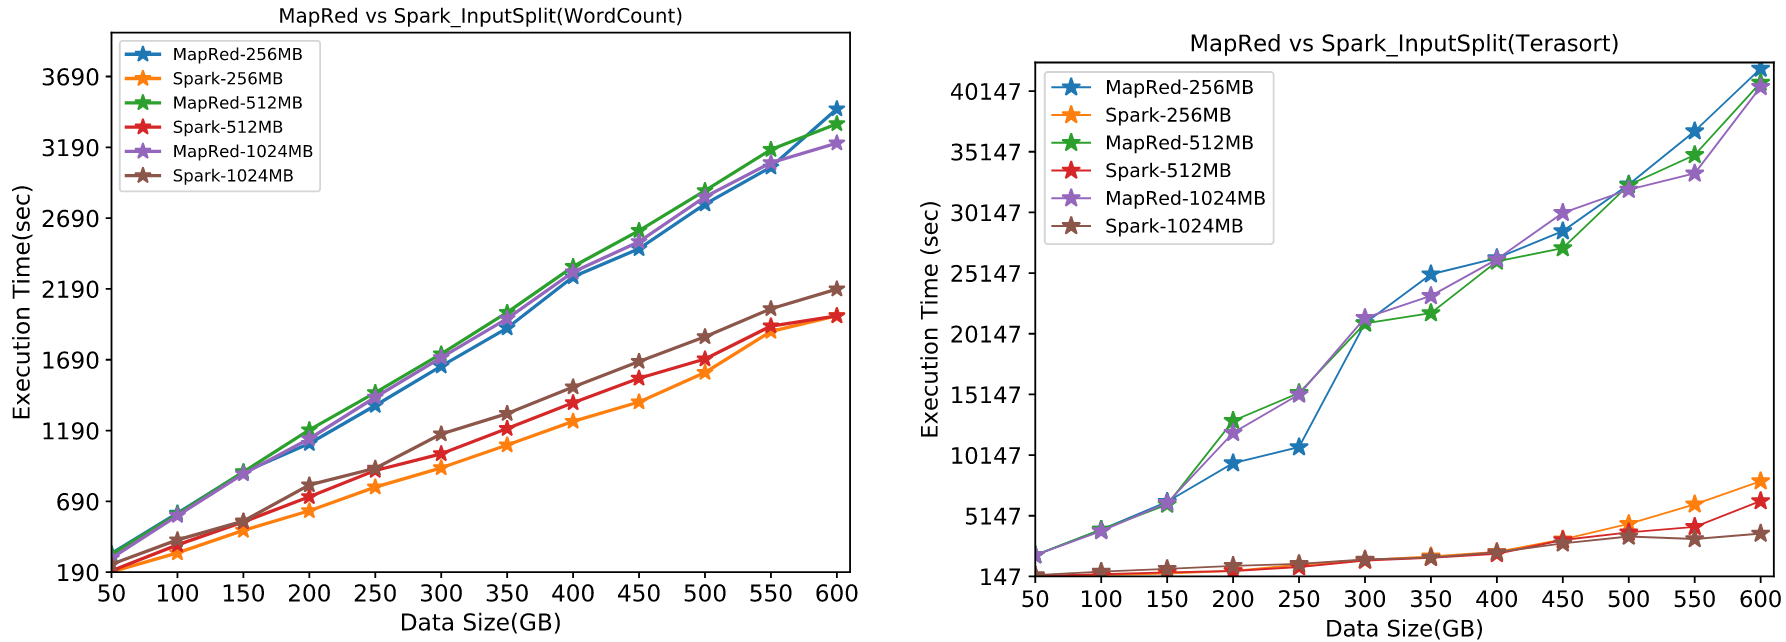
\includegraphics[width=\textwidth]{pics/MapRedvsSpark.png}
			\caption{Comparison of Hadoop and Spark with WordCount and TeraSort workload with varied input splits and shuffle tasks~\cite[14]{ahmed2020comprehensive}}
		\end{figure}
	}
\end{frame}

% \begin{frame}{Mögliche Fragen}
% 	\begin{itemize}
% 		\item Was passiert wenn der komplette Adressraum belegt ist?
% 		\item Wie können bereits erzeugte Daten geschützt werden?
% 		\item Betreibt nicht jeder Computer In-Memory Processing?
% 	\end{itemize}
% \end{frame}
